\section{L'avantage du mode incrémental dans Best/KBest}\label{sec:valid:perfs:prefs}
Nous avons vu dans le chapitre~\ref{chap:valid:domvision} que nous pouvons introduire des opérateurs de préférences contextuelles. Cette section présente les algorithmes que nous avons développés pour les opérateurs \textbf{Best} et \textbf{KBest}. Ces opérateurs nécessitent de connaître la hiérarchie des n-uplets déduite d'un ensemble de préférences. Cette hiérarchie est déduite du \textit{graphe de préférence} \textit{GP}. Nous présentons ci-après deux algorithmes pour la gestion du graphe ainsi qu'une étude des performances pour sélectionner le meilleur algorithme.

\subsection{Le graphe de préférence}
L'ordre de préférence entre deux n-uplets $t_1$ et $t_2$ selon une règle $\varphi$ est construit à partir d'une fonction $Com\-pare(t_1,t_2,\varphi_k)$ qui retourne $\emptyset$ si $t_1$ et $t_2$ sont incomparables, 1 si $t_1$ est préféré à $t_2$ et $-1$ sinon. L'algorithme~\ref{algo:comparT} étend la comparaison à une théorie $\Gamma$. Cette dernière utilise un ensemble de règles pour calculer l'ordre de préférence mais ne calcule par la clôture transitive.

\textbf{Graphe de préférence : }
Les opérateurs \textbf{Best} et \textbf{KBest} sont appliqués sur un ensemble de n-uplets $TS$ et ont besoin du graphe de préférence relatif à $TS$.
Pour son implémentation, nous avons adopté la structure $Graph(Next, Prec, Src)$ définie comme suit:
 $Next$ associe chaque n-uplet à la liste des n-uplets \textbf{qu'il domine}.
 $Prec$ associe chaque n-uplet à la liste des n-uplets \textbf{qui le dominent}.
 $Src$ est l'ensemble des n-uplets non-dominés, représentant la source du graphe.
Afin de fournir de bonnes performances, les implémentations de ces structures sont des \textit{hash-sets} ou \textit{hash-maps}.

La construction et la mise à jour du graphe utilisent des méthodes \textit{Graph.Insert} et \textit{Graph.Delete}. Pour insérer un n-uplet dans un graphe, la méthode \textit{Graph.Insert} itère sur les nœuds du graphe pour mettre à jour \textit{Next}, \textit{Prec} et l'ensemble \textit{Src}. Comme le coût de l'insertion et de suppression dans une structure hachée peut être considéré comme $\mathcal O(1)$, le coût global de l'insertion d'un n-uplet dans le graphe est de $\mathcal O(\abs G)$. Pour la suppression d'un n-uplet $s$ du graphe, la méthode \textit{Graph.Delete} itère sur les nœuds connectés à $s$. Le coût est de $\mathcal O(\mathrm{deg}(s))$.

Pour une théorie de préférences $\Gamma$ donnée et un ensemble de n-uplets $TS$, la construction du graphe de préférences complet est réalisée par l'algorithme~\ref{algo:create}.

\subsection{Calcul de Best et KBest}
Par définition, le graphe inclut l'ensemble $Src$ qui contient les n-uplets les plus préférés. L'ensemble $Src$ est le résultat de l'opérateur \textit{Best}. Toutefois, l'algorithme peut-être optimisé en évitant de construire complètement \textit{GP}. La méthode $Graphe.Insert$ peut être optimisée pour tenir compte de cela. 
La complexité est alors réduite à $\mathcal O(\abs{Src})$. La complexité de $Best(R)(b)$ devient $\mathcal O(NS)$ où $N = \abs{R(b)}$ et $S=\abs{Best(R)(t)}$.

L'algorithme principal utilisé pour calculer $KBest$ à partir du \textit{GP} est un tri topologique de Kahn limité aux $k$ premiers résultats. Voir l'algorithme~\ref{alg:kbest}.

\subsection{Evaluation incrémentale du GP}
Cette section présente un algorithme pour le calcul incrémental de \textit{GP}. Le fait que les requêtes avec préférences sur les flux s'expriment sur des séquences de fenêtres motive cette méthode. Il est nécessaire de construire le \textit{GP} pour l'ensemble des n-uplet de la fenêtre \textit{courante}. Comme deux fenêtres consécutives peuvent se superposer, le nouveau \textit{GP} peut être construit par mise à jour incrémentale du graphe \textit{courant}. 

Supposons que $\delta_R^{-}$ contienne les n-uplets \textit{sortants} de la fenêtre et $\delta_R^{+}$ contienne ceux qui \textit{rentrent} dans la nouvelle fenêtre. Il n'y a pas d'intersection entre ces deux ensembles. Ces ensembles sont utilisés par l'algorithme~\ref{algo:update} pour construire le \textit{GP} de la nouvelle fenêtre à partir du \textit{GP} de la précédente. 

Il est important de noter que l'approche incrémentale est intéressante si la différence entre deux graphes successifs est faible comparé à la taille totale du graphe. Dans un tel cas, une grande proportion du \textit{GP} est réutilisée. Dans le cas contraire, la création du \textit{GP} \textit{de zéro} est meilleure. Le tableau~\ref{tab:valid:perfs:prefs:complexity} résume l'ensemble des complexités algorithmiques.

\begin{table}[p]
\noindent
\begin{minipage}{0.55\textwidth}
\small
\begin{algorithm}[H]\caption{Calcule KBest$(R)(t)$}\label{alg:kbest}
\dontprintsemicolon
\KwData{La structure GP, $k$ le nombre d'n-uplet demandé}
Res $\gets $ \textbf{new TreeSet}$()$ \tcp{Ensemble ordonné}
\If{$k < \abs{Src}$}{\tcp{Src contient plus de $k$ n-uplets}
	$N \gets \abs{Src} - k$ \;\tcp{L'ordre position de Src est utilisé}
	\ForEach{$s\in Src$}{\tcp{ pour garder les $k$ n-uplets les plus récents}
		\lIf{$N = 0$}{Res.add$(s)$\;}
		\lElse{$N \gets N-1$\;}
	}
	\Return{Res}
}
NextLvl $\gets Src$; $id \gets 0$\;
PrecCount $\gets $ \textbf{new HashMap}()\;
\While{$id<k$ \textbf{and} $id < \abs{Src}+$Prec.count()}{
	\tcp{Buffer contient les n-uplets du même niveau}
	\If{Buffer = $\emptyset$}{
		\ForEach{$t\in $NextLvl}{
			Buffer.push$(t)$\;
		}
		NextLvl.clear()\;
	}
	$t\gets$ Buffer.pop()\;
	\ForEach{$s\in Next$.get$(t)$}{\tcp{Pour tout n-uplet dominé par $t$}
		$n\gets $PrecCount.get$(s)$\;
		\If{$n = $\textbf{null}}{$n=$Prec.get$(s)$.size()\;}
		\If{$n=1$}{
			NextLvl.add$(s)$\;\tcp{$s$ fait parti du prochain niveau}
		} \lElse {
			PrecCount.put$(s,n-1)$\;\tcp{Il n'y a plus de nœud dans cet ensemble}
		}
	}
	Res.add$(t)$\;
}
\Return{Res}
\end{algorithm}
\end{minipage}
\begin{minipage}{0.45\textwidth}
\small

\begin{algorithm}[H]\caption{ComparT$(t_1,t_2,\Gamma)$}\label{algo:comparT}
\dontprintsemicolon
%\begin{algorithmic}
%\KwIn{$t_1$ and $t_2$ two tuples from $R$}
\KwData{$\Gamma = \{\varphi_1,...,\varphi_k\}$ une théorie}
\KwResult{$\{1,-1,\emptyset\}$, \\ \quad resp. $\{t_1 >_{\Gamma} t_2$, $t_1 <_{\Gamma} t_2$, inc.$\}$}
\ForEach {$\varphi_k \in \Gamma$}{
	$r\gets Compare(t_1,t_2,\varphi_k)$\;
\lIf{$r \neq \emptyset$}{
\Return{$r$}
}
}
\Return{$\emptyset$}
%\end{algorithmic}
\end{algorithm}

\vspace{1cm}
\begin{algorithm}[H]\caption{Créer GP}\label{algo:create}
\dontprintsemicolon
\KwIn{$TS$ un ensemble d'n-uplets}
\KwData{La structure de GP}
\lForEach{$s\in TS$}{
	$Graph.$insert$(s)$\;
}
\end{algorithm}

\vspace{1cm}
\begin{algorithm}[H]\caption{GP incrémental}\label{algo:update}
\dontprintsemicolon
\KwIn{$\delta_R^{-}(t,i)$ and $\delta_R^{+}(t,i)$}
\KwData{La structure du GP}
\lForEach{$s\in \delta_R^{-}(t,i)$}{
	$Graph.$Delete$(s)$\;
}
\lForEach{$s\in \delta_R^{+}(t,i)$}{
	$Graph.$Insert$(s)$\;
}
\end{algorithm}

\vspace{1cm}
\begin{tabular}{rcc}
& Créer GP & GP Incrémental\\ \noalign{\hrule height 1pt}
Best \quad &\quad $\mathcal O(N.S)$\quad & $\mathcal O(\Delta.N)$ \\
KBest \quad & $\mathcal O(N^2)$ & \quad $\mathcal O((\Delta+k)N)$ \quad\\ \noalign{\hrule height 1pt}
\end{tabular}
\caption{Best/KBest complexity}\label{tab:valid:perfs:prefs:complexity}
\end{minipage}
\end{table}

\subsection{Expérimentations pour la sélection du plan de requête}
Nous avons à notre disposition deux composants capables de calculer de manière incrémentale ou non les opérateurs de préférences contextuelles. Dans cette section, nous expérimentons pour sélectionner l'un ou l'autre choix.

L'expérience a été réalisé dans un cadre applicatif financier. Ainsi, $30,000$ n-uplets ont été collectés depuis des flux de cours d'actions\footnote{Fournit par le service Dukascopy's Data Export. Disponible à \url{http://www.dukascopy.com/swiss/english/data_feed/csv_data_export}}. Les préférences utilisés sont de la même complexité que celles présentés en section~\ref{sec:valid:domvision:architecture}. Soit $S$ un flux, la requête que nous analysons est la suivante : $${\bf KBest}_k(S[N \textrm{ slide } \Delta])$$

\begin{figure}[ht]
\subfigure[En variant $\Delta$ sur KBest (pour $N=500$)]{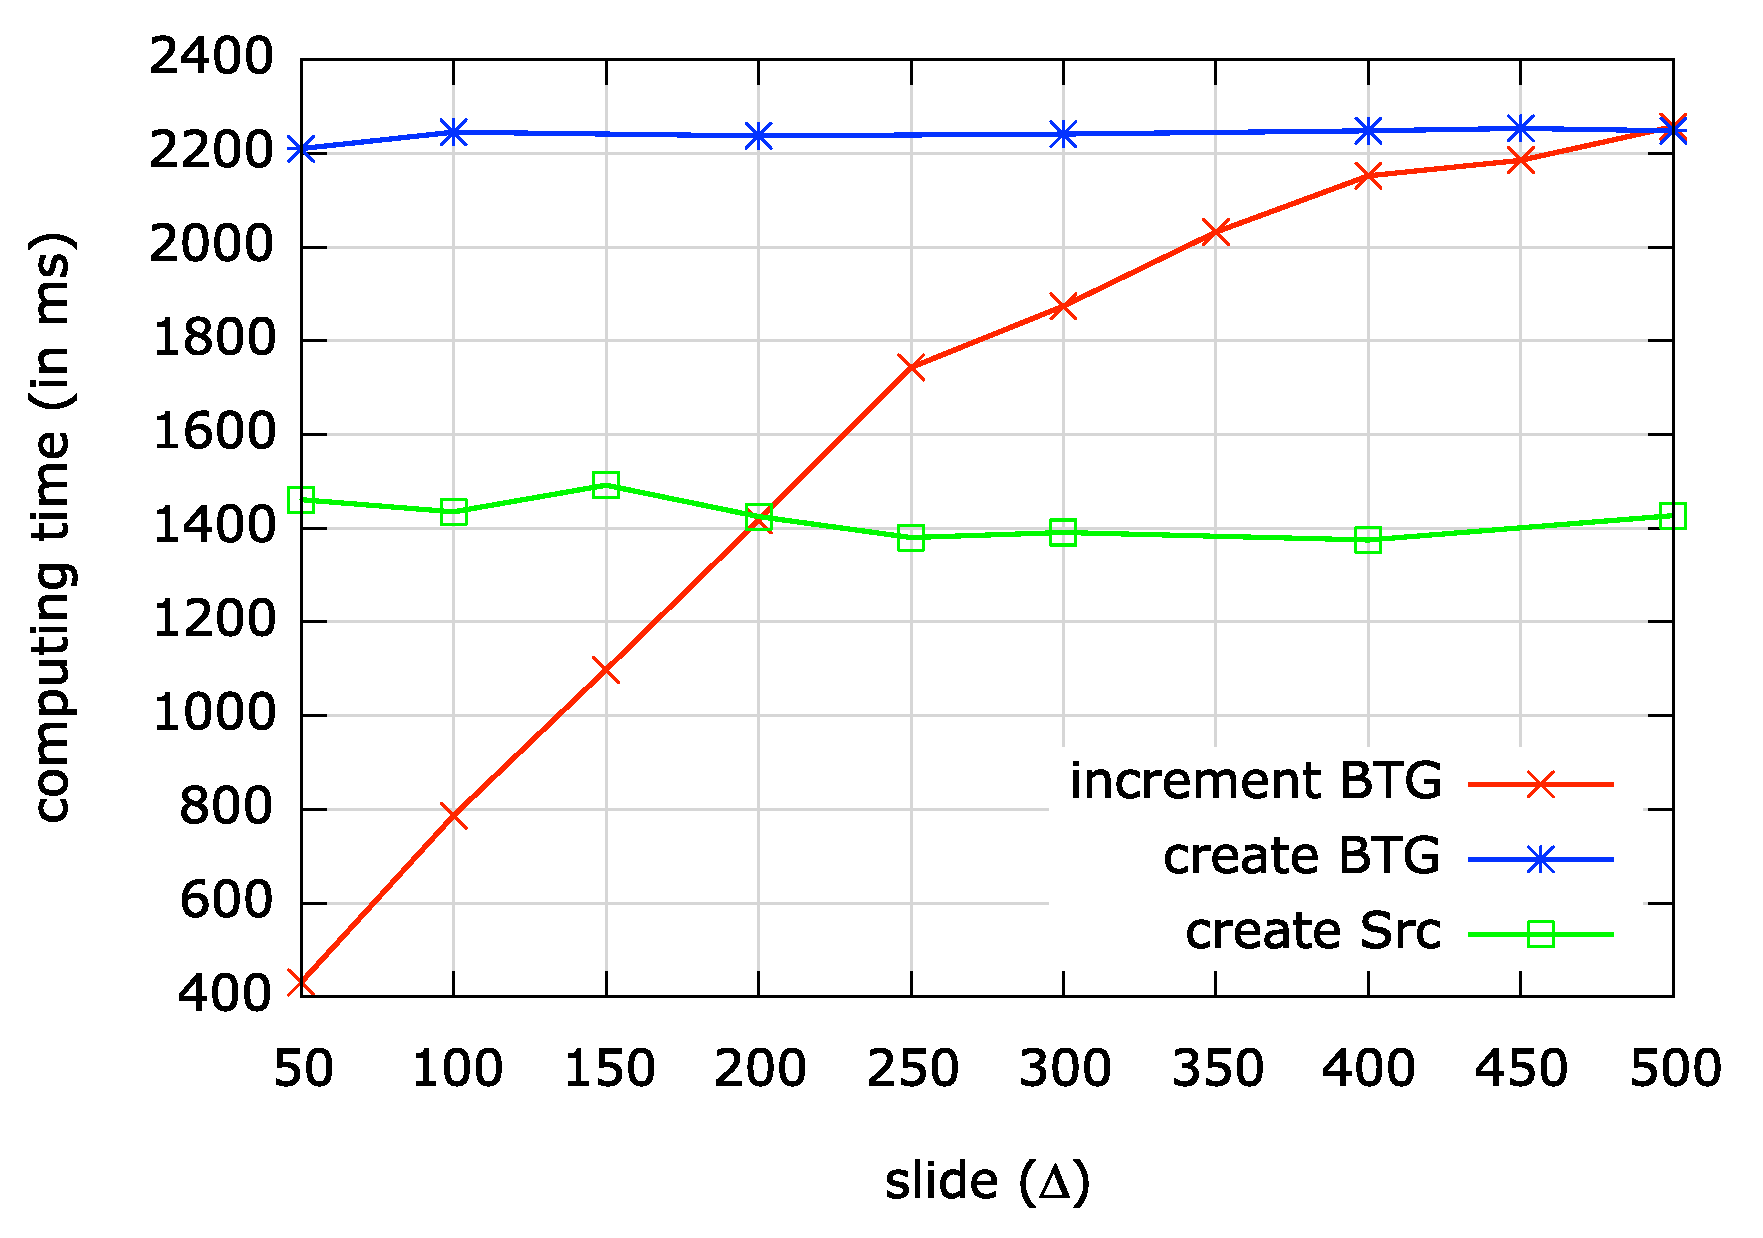
\includegraphics[width=0.48\linewidth]{valid-perfs-prefs-slide}\label{fig:prefxp-slide}}
\subfigure[En variant $N$ sur KBest (pour $\Delta=N$)]{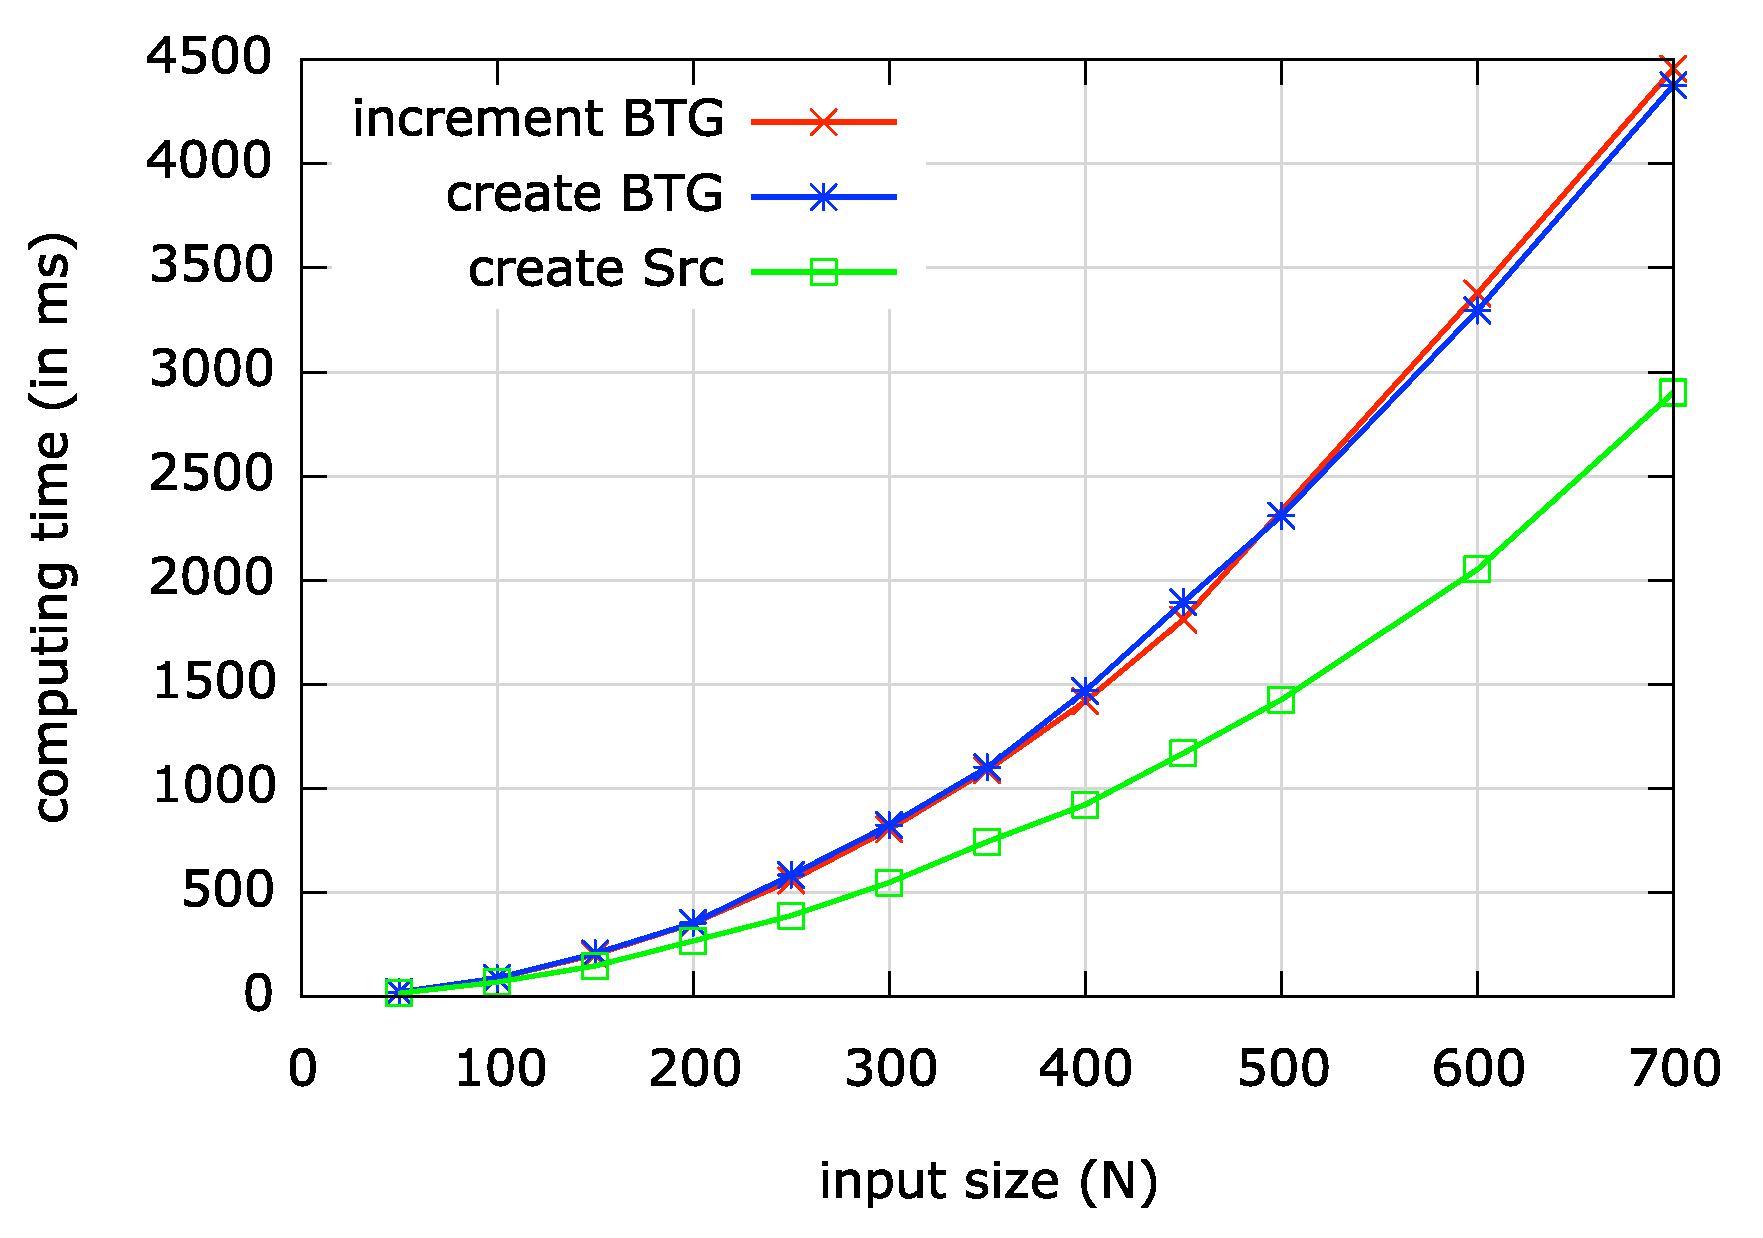
\includegraphics[width=0.48\linewidth]{valid-perfs-prefs-size}\label{fig:prefxp-size}}
\caption{Temps de calcul de \textit{Créer GP}, \textit{GP Incrémental} et de la maintenance de \textit{Src}}\label{fig:prefxp}
\end{figure}

\textbf{Résultats :} Les expérimentations montrent que le temps d'évaluation de \textbf{KBest} est dominé par la construction-mise à jour du \textit{GP}. Nous avons aussi observé que la structure du \textit{GP} d'une fenêtre à l'autre pouvait changer. La profondeur maximale du graphe varie de 2 à 6 et le nombre de n-uplets non-dominés varie de $1$ à $N$. Les grands changements de structures correspondent aux pires cas de l'algorithme incrémental. La figure~\ref{fig:prefxp-slide} montre le temps de calcul des deux algorithmes du \textit{GP} : \textit{créer} et \textit{incrémental}. Elle indique aussi le temps nécessaire au calcul réduit de la maintenance de \textit{Src}, qui est directement utilisée pour l'opérateur \textbf{Best}. 

Durant les expérimentations, nous avons utilisé plusieurs tailles de fenêtres $N$ et de taux $\Delta$. Nous remarquons que les changements de taux de mise à jour n'impactent pas le temps de création du \textit{GP}, tandis que l'algorithme incrémental obtient un gain de 6 pour un ration $N/\Delta=10$. Étonnement, les deux algorithmes du \textit{GP} se comportent de la même façon lorsque $\Delta\sim N$, ce qui correspond au cas où il n'y a pas ou peu d'intersections entre les fenêtres successives. Cela indique que dans la version incrémentale, les suppressions dans le \textit{BTG} prennent peu de temps comparé aux insertions. Ceci est notamment dû au fait que l'insertion nécessite l'évaluation des comparaisons (coûteuses dans notre cadre expérimental). Le coût de ces suppressions peut aussi être augmenté dans le cas où le \textit{GP} est un graphe fortement connexe, ce qui est difficile à trouver dans la pratique.

La variation de la taille de la fenêtre (figure~\ref{fig:prefxp-size} avec $\Delta=N$) montre que le comportement n'est pas impacté par le nombre d'n-uplets impliqués. Comme prévu, l'évolution semble quadratique selon $N$ et l'approche incrémentale suit strictement la performance de l'algorithme de création.

Nous pouvons désormais intégrer notre composant incrémental à l'intérieur d'Astronef par la création des deux règles suivantes :
\begin{lstlisting}[language=PrologAstral]
dynamicoperator([kbest,B,[C]]):- !,
    map_get(B, "incremental", "true", "true"), % Mode incremental par defaut
    dynamicoperator(C). % Si le noeud fils est aussi incremental

implrules([kbest,B,_,_], "DynamicKBest"):- isdynamic(B), !.
\end{lstlisting}
Pour plus de complétude, nous pourrions établir une règle disant que si nous sommes dans le cas $k=-1$ (i.e. \textbf{Best}) et que le ratio $N/\Delta$ de la description de fenêtre, s'il y en a une, est inférieur à 2 : alors nous devons utiliser l'opérateur \textbf{Best} non-incrémental.
